\subsection{Backpropagation}
Now that we have the model and its basic structure and parameters, we'll look into how to train it.

Our \textbf{first step in training} is the random assignment of weights and then the measurement of the error.
\begin{align*}
  &Error\left(\cv{x}, \cv{t}, \cv{w}\right) = \sum_{k=1}^N\frac{1}{2}\left(y_k - t_k\right)^2\\
  &{\footnotesize\text{With } \begin{array}{rl}
    \cv{x}:&\text{Input from training set}\\
    \cv{t}:&\text{Labels (target values)}\\
    \cv{y}:&\text{Calculated output with the help of }\cv{w}
  \end{array}\text{ all vectors of size }N}
\end{align*}

Our \textbf{training goal} is to lower the error in each training episode by changing the weights. But in which direction should we change which weight?
\begin{itemize}
  \item We have the same problem as before, and again we choose the steepest way down. The direction is known since we have the derivative of the function.
  \item But for our FNN, we have many weights. We need to pick a suitable step size, and we should do the update for all instances. For efficiency, this can be done in smaller batches.
\end{itemize}

So basically, we again apply gradient descent. But, when having thousands of neurons and millions of connections, the descent is performed in a space with millions or even billions of dimensions. To calculate how to nudge the weights, we therefore introduce the Neural Network Training Algorithm, better known as \textbf{Backpropagation}\sidenote{Backpropagation} algorithm. It consists of the repetition of two passes:
\begin{itemize}
  \item First, we have the \textbf{Forward pass}\sidenote{Forward pass}:
  \begin{enumerate}
    \item The network is activated on one example.
    \item Based on the calculated output, the \textit{error of neurons of the output layer} is computed.
  \end{enumerate}
  \item Second, we have the \textbf{Backward pass}\sidenote{Backward pass}:
  \begin{enumerate}
    \item Starting at the output layer, the \textit{error is propagated backwards} through the network (layer by layer)
    \begin{note}\begin{itemize}
      \item Recursively computing local deviation of error for each layer.
      \item Use derivatives to preview the effect of a small change.
    \end{itemize}\end{note}
    \item Then the \textit{weights are updated} (also for hidden layers).
  \end{enumerate}
\end{itemize}

\begin{figure}[H]
  \centering
  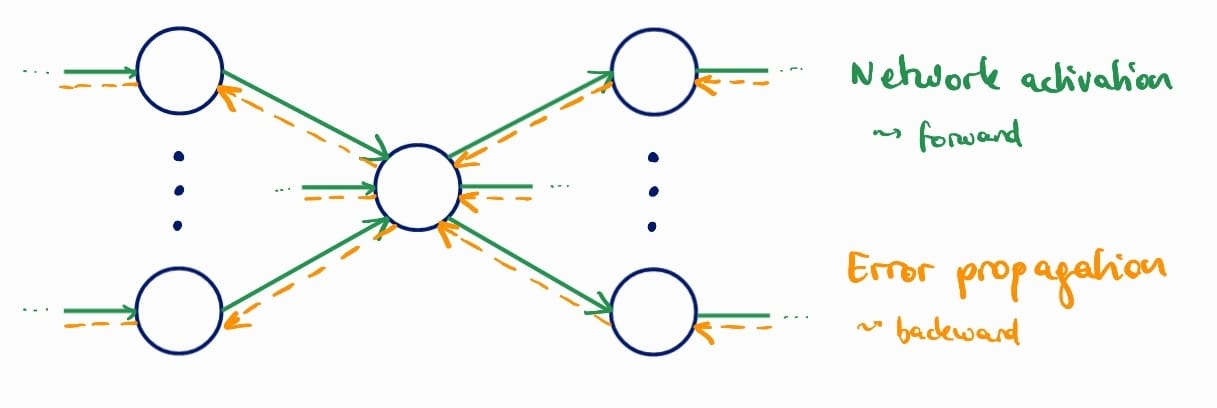
\includegraphics[width=0.8\textwidth]{assets/nn/bp__principle_steps.jpg}

  \caption{Backpropagation steps}
  \label{fig:6_bp_steps}
\end{figure}

To understand backpropagation, first, the concept of \textbf{derivatives} needs to be established:
\begin{align*}
  \left.\frac{d f(x)}{dx}\right|_{x=a} \text{ gives the slope of the curve } f \text{ at }x=a
\end{align*}
\begin{table}[h]
  \footnotesize
  \renewcommand{\arraystretch}{1.5}
  \centering
  \begin{subfigure}{0.45\textwidth}
  \begin{tabular}{|l|c|c|}
    \hline
    \textbf{Common Functions} & $f(x)$ & $\frac{d}{dx} f(x)$ \\
    \hline
    Constant & $c$ & $0$ \\
    Line & $x$ & $1$ \\
    Line & $ax$ & $a$ \\
    Square & $x^2$ & $2x$ \\
    Square Root & $\sqrt{x}$ & $\frac{1}{2}x^{-\frac{1}{2}}$ \\
    Exponential & $e^x$ & $e^x$ \\
    Exponential & $a^x$ & $\ln(a) \cdot a^x$ \\
    Logarithms & $\ln(x)$ & $\frac{1}{x}$ \\
    Logarithms & $\log_a(x)$ & $\frac{1}{x \ln(a)}$ \\
    Trigonometry & $\sin(x)$ & $\cos(x)$ \\
    Trigonometry & $\cos(x)$ & $-\sin(x)$ \\
    Trigonometry & $\tan(x)$ & $\sec^2(x)$ \\
    Inverse Trigonometry & $\sin^{-1}(x)$ & $\frac{1}{\sqrt{1-x^2}}$ \\
    Inverse Trigonometry & $\cos^{-1}(x)$ & $-\frac{1}{\sqrt{1-x^2}}$ \\
    Inverse Trigonometry & $\tan^{-1}(x)$ & $\frac{1}{1+x^2}$ \\
    \hline
  \end{tabular}
  \end{subfigure}
  \hspace{0.05\textwidth}  
  \begin{subfigure}{0.45\textwidth}
  \begin{tabular}{|l|c|c|}
    \hline
    \textbf{Rules} & $f(x)$ & $\frac{d}{dx} f(x)$  \\
    \hline
    Multiplication (const.) & $cf$ & $cf'$ \\
    Power Rule & $x^n$ & $nx^{n-1}$ \\
    Sum Rule & $f + g$ & $f' + g'$ \\
    Difference Rule & $f - g$ & $f' - g'$ \\
    Product Rule & $fg$ & $fg' + f'g$ \\
    Quotient Rule & $\frac{f}{g}$ & $\frac{f'g - g'f}{g^2}$ \\
    Reciprocal Rule & $\frac{1}{f}$ & $-\frac{f'}{f^2}$ \\
    \hline
    Chain Rule & $f \circ g$ & $(f' \circ g) \cdot g'$ \\
    Chain Rule & $f(g(x))$ & $f'(g(x)) \cdot g'(x)$ \\
    Chain Rule & $\frac{dy}{dx}$ & $\frac{dy}{du} \cdot \frac{du}{dx}$ \\
    \hline
  \end{tabular}
\end{subfigure}
  
  \renewcommand{\arraystretch}{1}
\end{table}

Consider the functions and variables we saw before for the two-layer FNN:\sidenote{$y_k$, $y_j$, $a_j$, $w_{ij}$}
\begin{align*}
  y_k(\cv{x}, \cv{w}) &= f\left( \sum_{j=0}^M w_{ik}^{(2)} z_j \right) \quad \text{for }1\leq k\leq N\\
  z_j &= h(a_j) = \sigma(a_j) = \frac{1}{1+\exp(-a_j)}\\
  a_j &= \sum_{i=0}^D w_{ij}^{(1)} x_i
\end{align*}

We'll calculate the weight update function for one single neuron $j$ regarded in isolation. 

\begin{figure}[H]
  \centering
  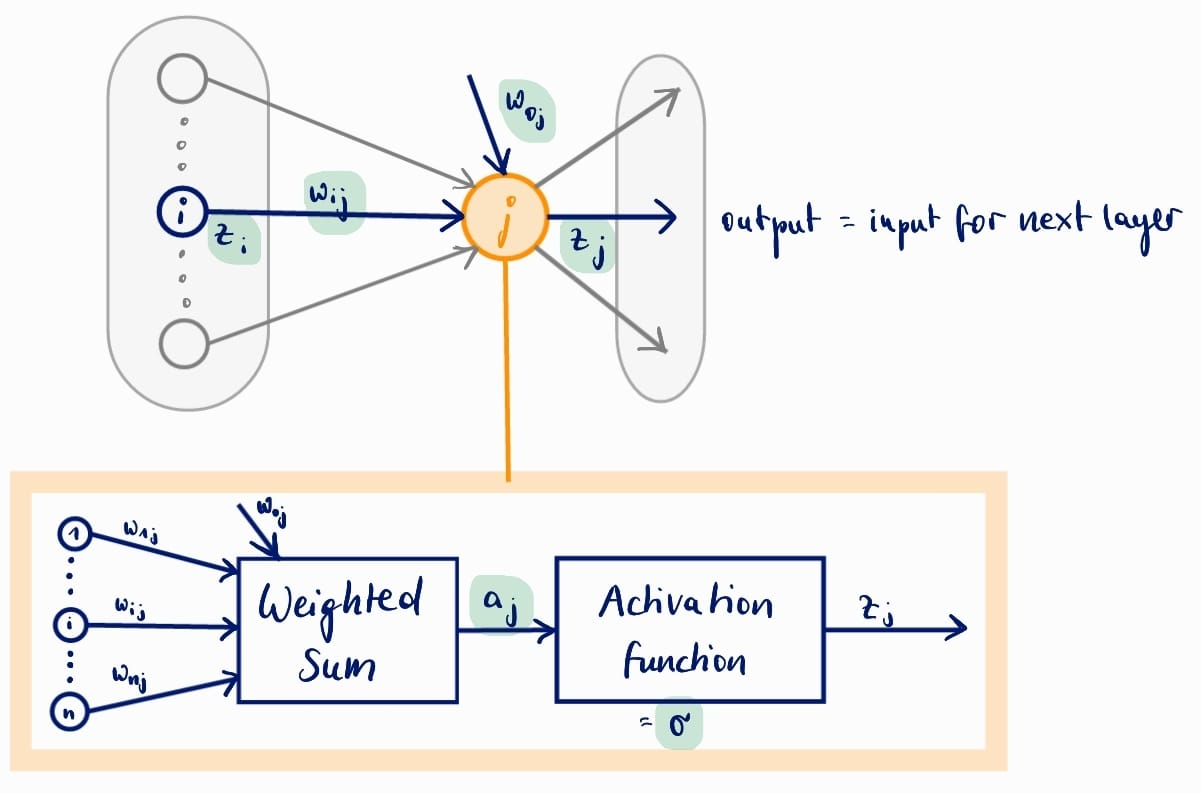
\includegraphics[width=0.7\textwidth]{assets/nn/bp__isolated_neuron.jpg}

  \caption{Isolated neuron components}
  \label{fig:6_bp_isolated_neuron}
\end{figure}

Each neuron in the hidden layers as well as in the output layer takes its input, sums them up with weights, and then applies the activation function to it. Here, we chose the sigmoid (logistic) function. Generally, there are different activation functions $h$ that can be used. But important for the backpropagation algorithm is that $h$ is differentiable:
\begin{itemize}
  \item Reason: we use the derivation of the error function, which is a variant of the gradient descent used for regression
  \item Figure \ref{fig:6_bp_h} shows different activation functions, from which only the Sigmoid function is suitable for backpropagation
\end{itemize}

\begin{figure}[H]
  \centering
  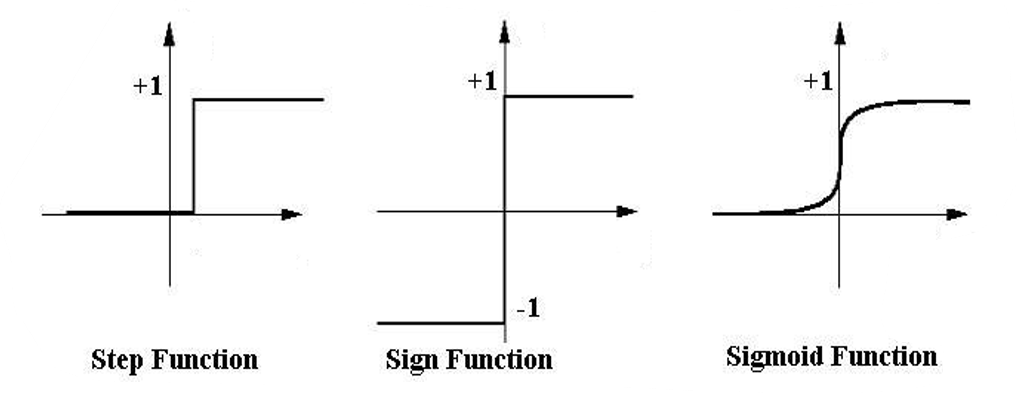
\includegraphics[width=0.6\textwidth]{assets/nn/bp__sigmoid.png}

  \caption{Activation functions (sigmoid)}
  \label{fig:6_bp_h}
\end{figure}

What we now want to do with our isolated neuron $j$, whichever one this is, is to minimize the general error by nudging all its regarding weights $w_{ij}$, so we want to calculate $\frac{\partial Error}{\partial w_{ij}}$.
\begin{itemize}
  \item Just quick note: for $w_{0j}$ we have $z_0 = 1$ and hence $w_{0j}z_0 = 1$
  \item Our error is again defined as: $Error = \frac{1}{2}\sum_{\text{instances}}\sum_k (y_k - t_k)^2$ where the sum over instances is related to batch updating and epochs (in detail later)
  \item Important to mention about the indices: technically, we need to include the layer number (dropped here for simplicity)
\end{itemize}

Assume we notch the error definition a bit, and not regard the output of the whole NN but instead of a single layer. So we have:
\begin{align*}
  Error = \frac{1}{2}\sum_k (z_k - t_k)^2
\end{align*}

Further, we define $E_{ij} := -\frac{\partial Error}{\partial w_{ij}}$ to indicate the direction of the desired change for $w_{ij}$. With that, we define our update:
\begin{align*}
  w_{ij}^{\text{new}} := w_{ij}^{\text{old}} + \partial w_{ij} = w_{ij}^{\text{old}} + \underbrace{l}_{\text{learning rate}}\cdot E_{ij}
\end{align*}
\begin{itemize}
  \item This introduces also a scaling parameter, precisely the learning rate $l$ (similar to step size)
  \item The $\partial w_{ij}$ aims to reduce the error
\end{itemize}

When we look at all our definitions, we can see that our $w_{ij}$ only has effects "downstream" the network activation flow. We therefore can apply the chain rule. For that, we again introduce a new variable $E_j = -\frac{\partial Error}{\partial a_j}$.
\begin{align*}
  E_j &= -\frac{\partial Error}{\partial a_j} = -\frac{\partial Error}{\partial z_j}\frac{\partial z_j}{\partial a_j} = -\frac{\partial Error}{\partial z_j} \big(\underbrace{\sigma(a_j)}_{= \frac{1}{1+e^{-a_j}}}\big)'\\
  &= -\frac{\partial Error}{\partial z_j} \cdot (-1)\frac{1}{(1+e^{-a_j})^2}\underbrace{e^{-a_j}\cdot(-1)}_{= (1+e^{-a_j})'} \\
  &= -\frac{\partial Error}{\partial z_j} \underbrace{\frac{1}{1+e^{-a_j}}}_{=z_j}\underbrace{\frac{e^{-a_j}}{1+e^{-a_j}}}_{=\left(1-\frac{1}{1+e^{-a_j}}\right)} = -\frac{\partial Error}{\partial z_j} z_j (1-z_j)\\\\
  E_{ij} &= -\frac{\partial Error}{\partial w_{ij}} = -\frac{\partial Error}{\partial a_j}\frac{\partial a_j}{\partial w_{ij}} = E_j \frac{\partial a_j}{\partial w_{ij}}\\
  &= E_j \frac{\partial (\sum_{i^*} w_{i^*j}z_{i^*})}{\partial w_{ij}} = E_j \left(\underbrace{\sum_{i^*\neq i}\frac{\partial w_{i^*j}z_{i^*}}{\partial w_{ij}}}_{=0} + \underbrace{\frac{\partial w_{ij}z_i}{\partial w_{ij}}}_{=z_i}\right)\\
  &= E_j z_i
\end{align*}

The last computation we need to do is $-\frac{\partial Error}{\partial z_j}$. For this case, we have two cases:
\begin{enumerate}
  \item $j$ is in the \textbf{output layer}
  \begin{align*}
    &\implies & z_j = t_j\\
    &\implies & -\frac{\partial Error}{\partial z_j} &= -\frac{\partial \left( \frac{1}{2}\sum_{j^*} (z_{j^*} - t_{j^*})^2 \right)}{\partial z_j}\\
    &&& = - \frac{1}{2}\left( \underbrace{\sum_{j^*\neq j}(z_{j^*} - t_{j^*})^2}_{=0} + \underbrace{(z_{j} - t_{j})^2}_{=z_j - t_j} \right) = t_j - z_j\\
    &\implies & E_{ij} &= E_j z_i = -\frac{\partial Error}{\partial z_j} z_j (1-z_j) z_i = (t_j - z_j)  z_j (1-z_j) z_i \\
    &\implies & \Delta w_{ij} &= l\cdot z_i z_j (1-z_j)(t-z_j)\\
    &\text{And in particular} & \Delta w_{0j} &= l\cdot z_j (1-z_j)(t-z_j)
  \end{align*}
  \item $j$ is in a \textbf{hidden layer}, which means changes in $z_j$ impact all $a_k$ values in the next layer proportional to the connection weight.
  \begin{align*}
    &\implies & -\frac{\partial Error}{\partial z_j} &= -\sum_k \underbrace{\frac{\partial Error}{\partial a_k}}_{=-E_k} \frac{\partial a_k}{\partial z_j}\\
              &&& = -\sum_k -E_k \underbrace{\frac{\partial \sum_{j^*} w_{j^* k}z_{j^*}}{\partial z_j}}_{=\frac{\partial w_{jk}z_j}{\partial z_j} = w_{jk}}  = \sum_k w_{jk}E_k\\
    &\implies & E_j &= z_j (1-z_j)\sum_k w_{jk}E_k\\
    &\implies & E_{ij} &= z_i z_j (1-z_j)\sum_k w_{jk}E_k\\
    &\implies & \Delta w_{ij} &= l\cdot z_i z_j (1-z_j)\sum_k w_{jk}E_k\\
    &\text{And in particular} & \Delta w_{0j} &= l\cdot z_j (1-z_j)\sum_k w_{jk}E_k
  \end{align*}
\end{enumerate}

Summarized, we have explicit expressions for our updates:\sidenote{Weight update, $E_{ij}$, $E_{j}$, $\Delta w_{ij}$}
\begin{align*}
  w_{ij}^\text{new} &= w_{ij}^\text{old} + \Delta w_{ij} 
    && \begin{array}{l} \text{updated weight of connection from neuron } i \\ \text{to neuron } j \text{ based on some training instance} \end{array}\\
  \Delta w_{ij} &= l E_{ij} = l E_j z_i\\
  \Delta w_{j} &= l E_{j}\\
  E_{j} &= z_j (1-z_j) (t-z_j) 
    && \begin{array}{l} \text{\textbf{Case 1:}} \\ \text{neuron } j \text{ is in the output layer} \end{array}\\
  E_{j} &= z_j (1-z_j) \sum_k w_{jk} E_k
    && \begin{array}{l} \text{\textbf{Case 2:}} \\ \text{neuron } j \text{ is in a hidden layer} \end{array}\\
    &&& \,\text{ With scaling parameter } l \text{ as the learning rate}
\end{align*}

Next, we're gonna investigate the \textbf{learning rate}\sidenote{Learning rate $l$}, which is usually a constant between $0.0$ and $1.0$.
\begin{itemize}
  \item As a rule of thumb: $l=\frac{1}{r}$ with $r$ being the "round", so the number of iterations
  \item It can also help to start with bigger steps and end with smaller ones to help a quicker convergence while avoiding overshooting the target
  \item The choice of $l$ is similar to the choice of the step size in regression and SVMs
  \item Typical problem:
  \begin{align*}
    l \text{ too small}: & \text{ learning occurs at very slow pace}\\
    l \text{ too large}: & \text{ oscillation between inadequate solutions can occur}
  \end{align*}
\end{itemize}

An important thing to consider for backpropagation is \textbf{when to update}:
\begin{itemize}
  \item In the case of \textbf{instance updating}\sidenote{Instance updating} we update the NN for each instance (sample) individually.
  \item Contrary, when we apply \textbf{batch updating}\sidenote{Batch updating} the NN is updated for a subset (or all) of all training instances in one update action. \begin{note}So we have an error calculation based on the same weights for multiple instances\end{note}
  \item Best practice is using \textbf{mini batches}, where the size depends on the problem.
  \item Another important term is \textbf{epoch}\sidenote{Epoch}, which describes one complete consideration of all the training data.
\end{itemize}

Finally, there's also the consideration for the \textbf{termination}\sidenote{Termination} of the backpropagation algorithm. There are multiple termination criteria indicating to stop training.
\begin{itemize}
  \item All $\Delta w_{ij}$ in the previous epoch are small (below some specified threshold)
  \item Percentage of misclassified inputs in previous epoch is small
  \item Pre-specified number of epochs has expired
  \item In practice: Several hundreds of thousands of epochs may be required before weights are converging
\end{itemize}
